%!TEX root = ../thesis.tex
%*******************************************************************************
%*********************************** Experiment *****************************
%*******************************************************************************

\chapter{Experiment} 

\ifpdf
    \graphicspath{{chapter-experiment/Figs/Raster/}{chapter-experiment/Figs/PDF/}{chapter-experiment/Figs/}}
\else
    \graphicspath{{chapter-experiment/Figs/Vector/}{chapter-experiment/Figs/}}
\fi

One of Europe's first joint ventures in science~\cite{About:1997225}, CERN (Conseil Européen pour la Recherche Nucléaire) is the largest physics research facility in the world, bringing together more than \num[group-separator={,}]{12200} people from of 110 nationalities to work together and push the frontiers of science and technology. Located at the Franco-Swiss border near Geneva, CERN was founded in 1954 and nowadays counts 23 member states~\cite{About:1997225}. CERN's main research area is particle physics, hence why the organization operates a full complex of particle accelerators and detectors.

This chapter introduces the Large Hadron Collider (LHC), CERN's main particle accelerator, as well as the ATLAS experiment, in which the SUSY search presented in this work is embedded in.

\section{The Large Hadron Collider}\label{sec:lhc}

The LHC~\cite{Evans:1129806} is the largest particle accelerator situated at CERN. It is installed in a tunnel with $\SI{26.7}{\km}$ circumference, that was originally constructed from 1984 to 1989 for the Large Electron Positron (LEP) accelerator. The tunnel is situated on the Franco-Swiss border and wedged between the Jura mountains and lake Léman. It lies between $\SI{45}{\meter}$ (in the limestone of the Juar) and $\SI{170}{\meter}$ (in molasse rock) below the surface, resulting in a tilt of $1.4\%$ towards the lake.  While proton-proton ($pp$) collisions are the main operating mode of the LHC, its design also allows it to accelerate and collide heavy ions like lead and xenon. Since data from $pp$ collisions is used in this work, the following sections will mainly focus on this operating mode. As a particle-particle collider, the LHC obviously consists of two rings with counter-rotating beams, as opposed to particle-antiparticle colliders that only need a single ring. With an inner diameter of only $\SI{3.7}{\meter}$, the tunnel however simply too narrow to fit two separate proton rings. Instead the LHC is built in a twin bore design\footnote{Originally proposed by John Blewett at BNL for cost-saving measures of the Colliding Beam Accelerator~\cite{Evans:1129806}.}, housing two sets of coils and beam channels in a single magnetic and mechanical structure and cryostat~\cite{Evans:1129806}. While saving costs, this design has the disadvantage of both beams being magnetically coupled, thereby reducing flexibility of the machine. 

Before being injected into the LHC, protons are pre-accelerated by an injection chain built from multiple existing machines in CERN's accelerator complex, pictured in \cref{fig:accelerator_complex}. The injection chain consists of predecessor accelerators that have been upgraded in order to be able to handle the high luminosity and high energy requirements of the LHC. The protons for the LHC stem from a duoplasmatron source~\cite{Scrivens:1382102}, stripping electrons from hydrogen atoms through electric discharges between a hot anode and cathode. The $\SI{90}{\keV}$ protons are then accelerated by a radio frequency (RF) quadrupole to $\SI{750}{\keV}$ before being injected into Linac2\footnote{Originally built to replace Linac 1 in order to produce higher energetic proton beams, Linac 2 has been replaced by Linac 4 in 2020.}, a linear accelerator producing a beam of $\SI{50}{\MeV}$ protons through the use of RF cavities. The protons then enter a set of circular accelerators, the Proton Synchrotron Booster (PSB), the Proton Synchrotron (PS) and the Super Proton Synchrotron (SPS), creating a stepwise acceleration up to an energy of $\SI{450}{\GeV}$, which is the injection energy of the LHC. The LHC finally accelerates the protons up to nominal beam energy before colliding them. 

\begin{figure}
	\centering    
	\includegraphics[width=0.9\textwidth]{CCC-v2019-final-white}
	\caption[CERN accelerator complex]{CERN accelerator complex as of 2018~\cite{Mobs:2684277}.}
	\label{fig:accelerator_complex}
\end{figure}

The LHC is composed of eight straight sections and eight arcs. The eight straight sections each serve as interaction points (IP), either for particle detectors, or for machine hardware of the collider itself. The IPs are labelled clockwise, with IP 1 being closest to the CERN Meyrin site. Four of the eight IPs house the main particle physics experiments at the LHC, called ATLAS, CMS, ALICE and LHCb, covering a wide range of fundamental research. The two general purpose particle detectors ATLAS~\cite{Aad:2008zzm} and CMS~\cite{Chatrchyan:2008aa} are installed at IP 1 and IP 5, respectively. Both ATLAS and CMS are designed to perform high precision SM measurements including Higgs measurements as well as searches for BSM physics. Being very similar in terms of targeted phase space, ATLAS and CMS can be used to cross-check results of each other. ALICE~\cite{Aamodt:2008zz} is situated at IP 2 and specializes on heavy ion physics, studying the physics of quark-gluon plasma at high energy densities. Built in IP 8, LHCb~\cite{Alves:2008zz} targets $B$-physics and performs measurements of CP-violation. Apart from the four main experiments, three smaller experiments exist at the LHC: TOTEM, MoEDAL and LHCf. While TOTEM~\cite{Anelli:2008zza} and LHCf~\cite{Adriani:2006jd} study forwards physics close to CMS and ATLAS, respectively, MoEDAL~\cite{Pinfold:2009oia} searches for magnetic monopoles.

The remaining four IPs house accelerator equipment needed for operation of the LHC. Most of the collimation system is placed at IP 3 and IP 7, performing beam cleaning and machine protection through a series of beam intercepting devices, ensuring that no stray particles from experimental debris or beam halo can reach and damage other machine components. The acceleration of the beam itself is performed at IP 4 with two radio frequency (RF) systems, one for each LHC beam. The RF cavities operate at $\SI{400}{\MHz}$ and provide $\SI{8}{MV}$ during injection and $\SI{16}{MV}$ during coast~\cite{Evans:1129806}. Due to the RF acceleration, the accelerated protons are grouped in packages called \textit{bunches}, each containing roughly $10^{11}$ protons, with a bunch spacing of $\SI{25}{ns}$~\cite{Evans:1129806}. Each beam contains a total of 2808~\cite{Evans:1129806} bunches as design value. The remaining of the IPs, IP~6, houses the beam dumping system, allowing to horizontally deflect and fan out both beams into dump absorbers using fast-paced \textit{kicker} magnets. The two nitrogen-cooled dump absorbers each consist of a graphite core contained in a steel cylinder, surrounded by $\SI{750}{\tonne}$ of concrete and iron shielding~\cite{Bruning:782076}. Insertion of the beams from the SPS into the LHC happens at IP 2 and IP 8, close to the ALICE and LHCb experiments.

The eight arcs of the LHC are filled with dipole magnets built from superconducting NbTi Rutherford cables. The electromagnets are responsible for keeping the accelerated particles on their circular trajectory and are the limiting factor of the maximal centre-of-mass energy $\sqrt{s}$ of the LHC. In order to achieve the design energy of $\sqrt{s} = \SI{14}{\TeV}$~\cite{Bruning:782076}, the magnets have to create a field strength of $\SI{8.3}{T}$~\cite{Evans:1129806}. In order to sustain the electric currents needed for such high field strengths, the magnets need to be cooled down to $\SI{1.9}{K}$~\cite{Evans:1129806} using superfluid helium and operated in superconducting state. In addition to the dipole magnets, the arcs contain quadrupole magnets used to shape and focus the beams, as well as multipole magnets correcting and optimizing the beam trajectory. Quadrupole magnets are also used to reduce the beam size before and after IPs.

\subsection{Pileup}

\begin{figure}
	\centering
	\begin{subfigure}[b]{0.45\linewidth}
		\centering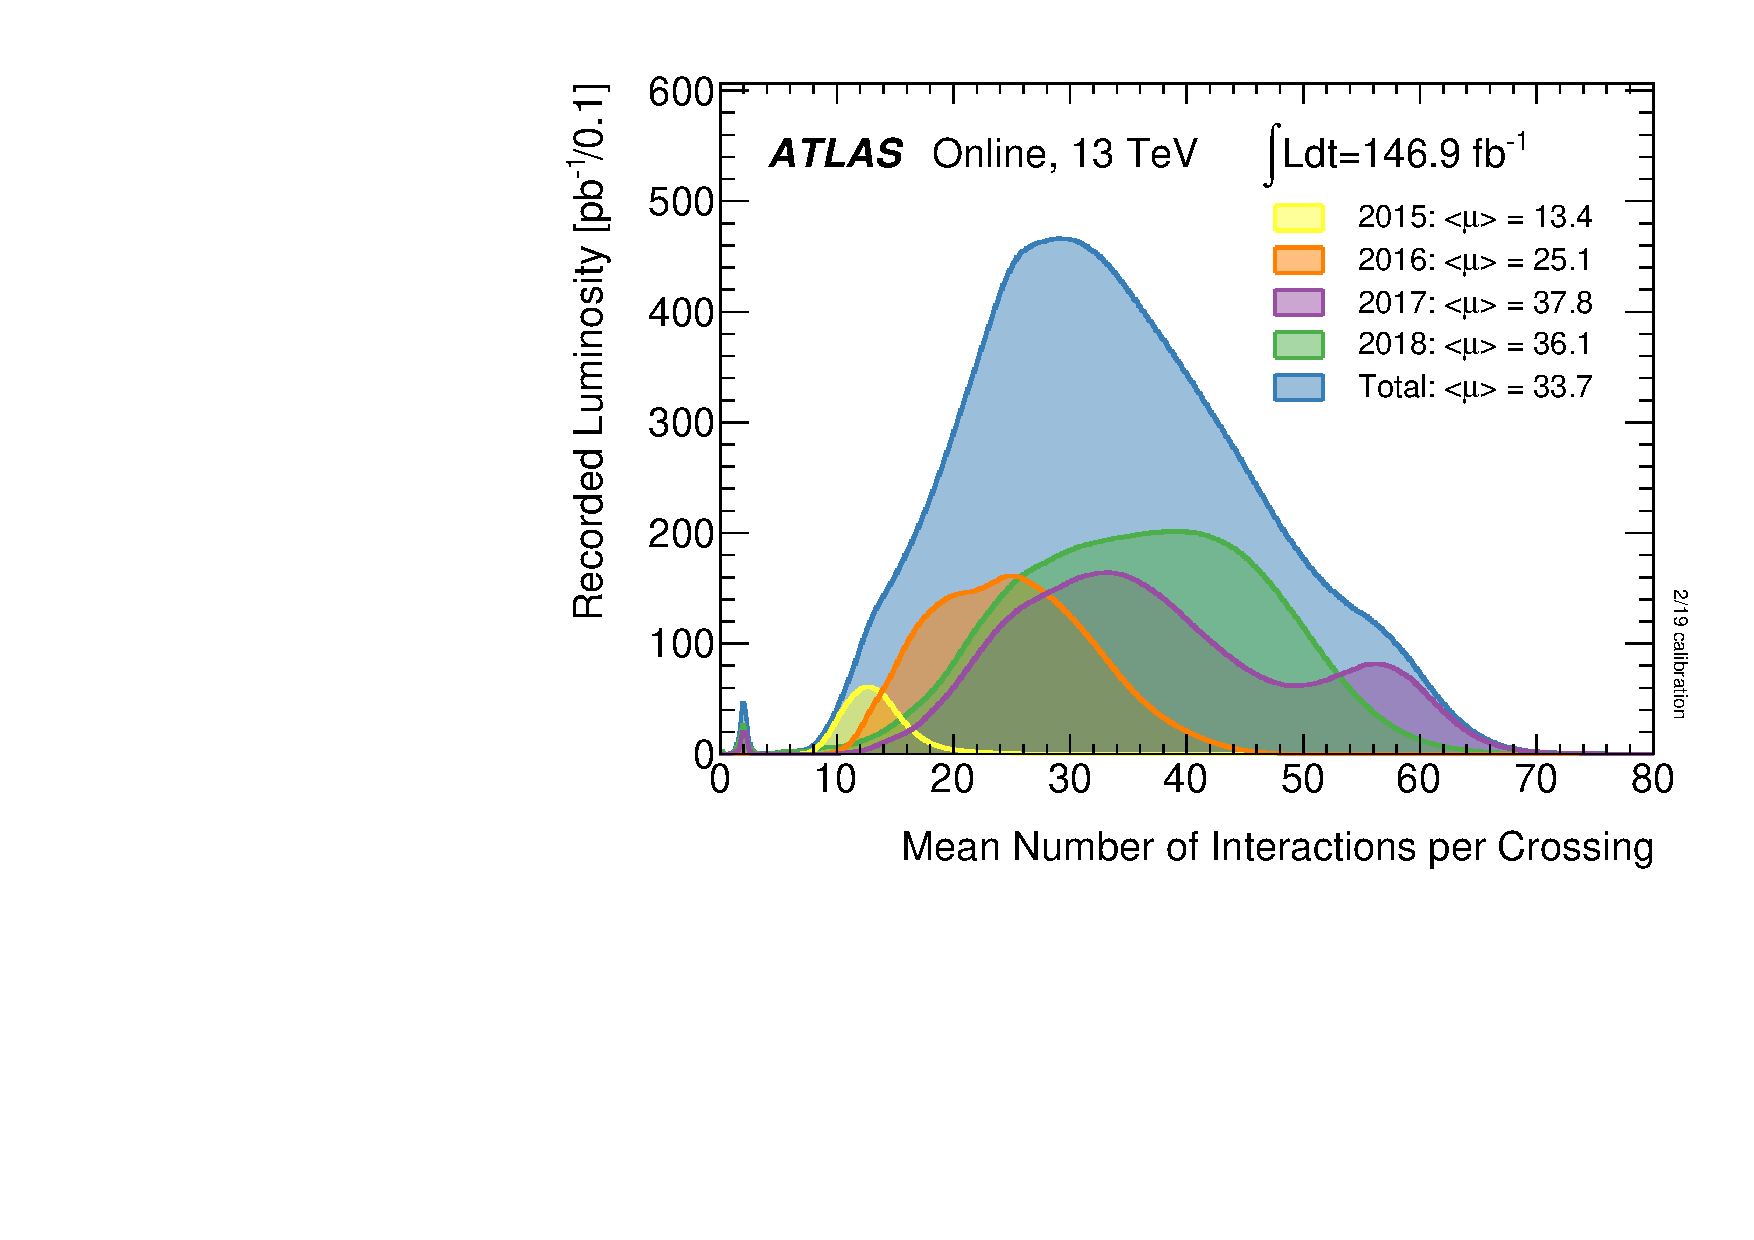
\includegraphics[width=\textwidth]{mu_2015_2018}
		\caption{Luminosity-weighted mean number of interactions per bunch crossing during Run~2 data-taking.\label{fig:mu_2015_2018}}
	\end{subfigure}%
	\begin{subfigure}[b]{0.45\linewidth}
		\centering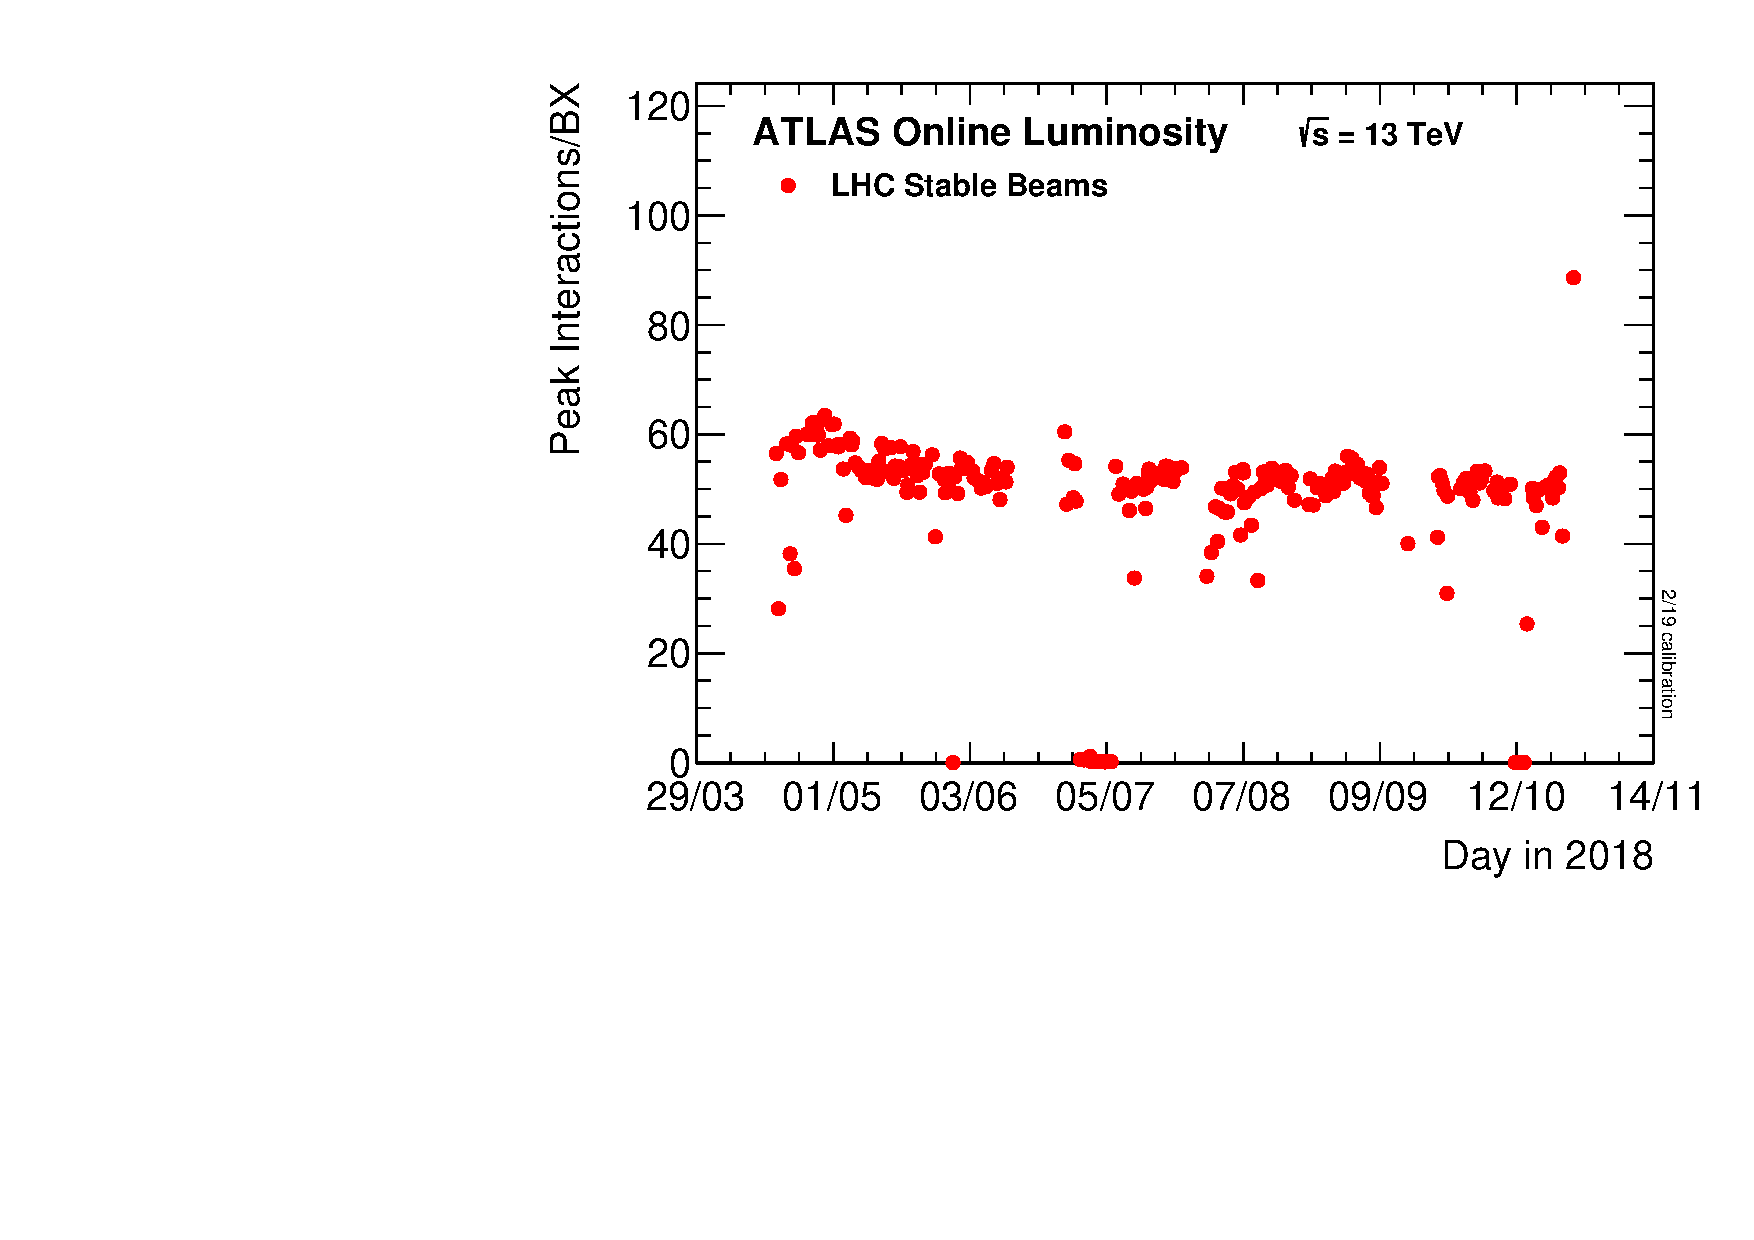
\includegraphics[width=\textwidth]{peakMuByFill}
		\caption{Peak mean number of interactions per bunch crossing for each fill during 2018.\label{fig:peakMuByFill}}
	\end{subfigure}%
	\caption{Number of interactions per bunch crossing recorded by the ATLAS detector~\cite{ATLAS:Run2}}\label{fig:mu_run2}
\end{figure}

Due to the high number of protons in each bunch, several $pp$ collisions occur at each bunch crossing. This leads to a phenomenon called \textit{pile-up}, where the recorded events not only contain information from the hard-scattering process of interest, but also remnants from additional, often low-energy, $pp$ collisions. During the Run~2 data-taking period, the mean number of inelastic $pp$ collisions per bunch crossing, $\mu$, has varied from roughly 10 to 70, with the majority of bunch crossings having a value of $\mu$ around 30. \Cref{fig:mu_2015_2018} shows the mean number of interactions per bunch crossing during the Run-2 data-taking period, weighted by luminosity. The peak number of interactions per bunch crossing $\mu_\mathrm{peak}$ per fill has been consistently around 50 during the 2018 data-taking (cf.~\cref{fig:peakMuByFill}).

Experimentally, pile-up can be divided into five major components~\cite{Marshall:2014mza}:
\begin{itemize}
	\item \textit{In-time} pile-up: multiple interactions during a single bunch crossing, of which not all will be interesting, as often with relatively low energy. If they can be resolved, the main hard-scattering event can still be isolated and studied.
	\item \textit{Out-of-time} pile-up: additional collisions occurring in bunch crossings before or after the main event of interest. This happens either due to read-out electronic integrating over longer time frames than the $\SI{25}{ns}$ bunch spacing, or detector components being sensitive to several bunch crossings.
	\item \textit{Cavern background}: gas of thermal neutrons and photons that typically fill the experimental caverns during a run of the LHC and tend to cause random hits in detector components.
	\item \textit{Beam halo events}: protons scraping an up-stream collimator, typically resulting in muons travelling parallel to the beam pip
	\item Beam gas events: collision events that originate from interactions between proton bunches and residual gas inside the beam pipe.
\end{itemize}
While the effects of cavern background can be mitigated through special pieces of shielding, beam halo and beam gas events leave signatures that can be recognized and removed. Signals from in-time and out-of-time pile-up create irreducible overlap with the events of interest, significantly impacting analyses, and thus need to be simulated~\cite{Marshall:2014mza}.

\subsection{Luminosity and data-taking}

\begin{figure}
	\centering
	\begin{subfigure}[b]{0.45\linewidth}
		\centering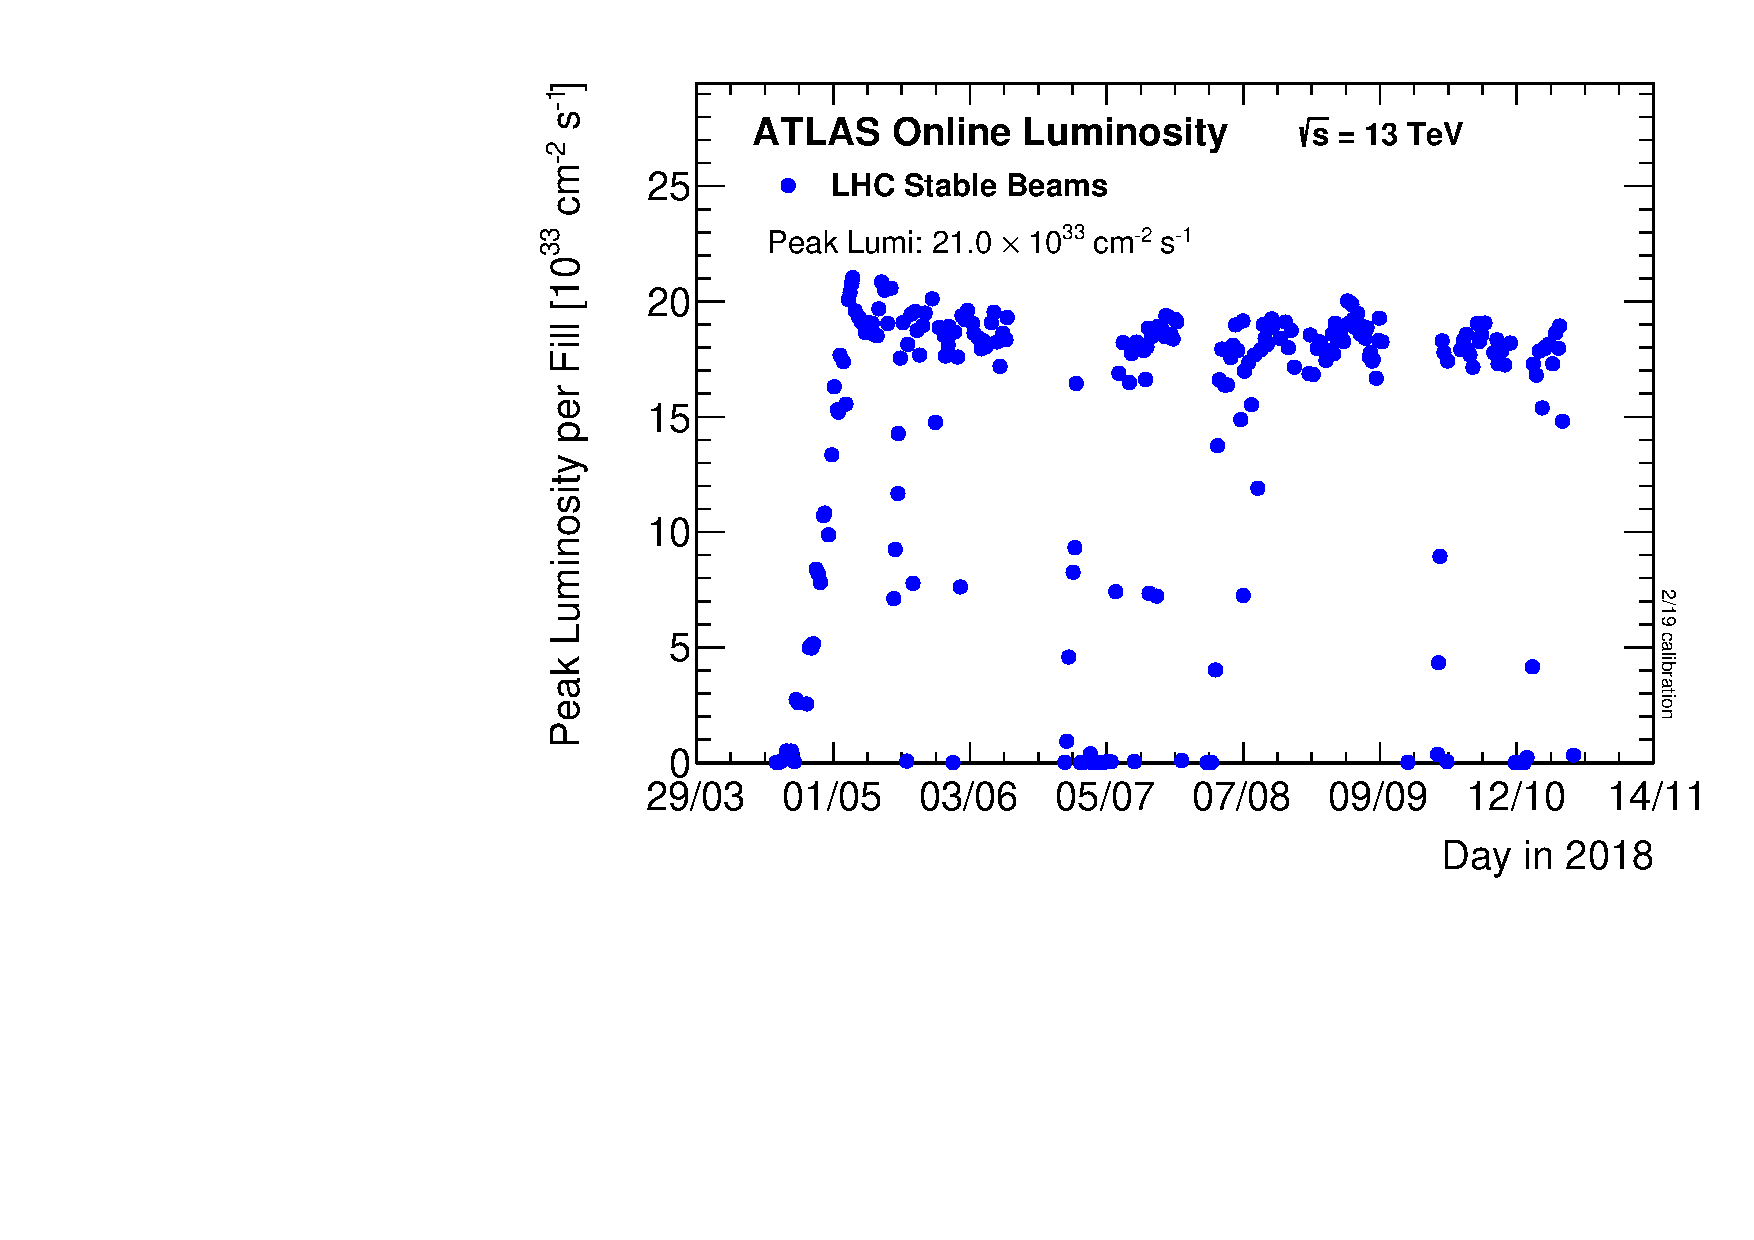
\includegraphics[width=\textwidth]{peakLumiByFill}
		\caption{\label{fig:peakLumiByFill}}
	\end{subfigure}%
	\begin{subfigure}[b]{0.45\linewidth}
		\centering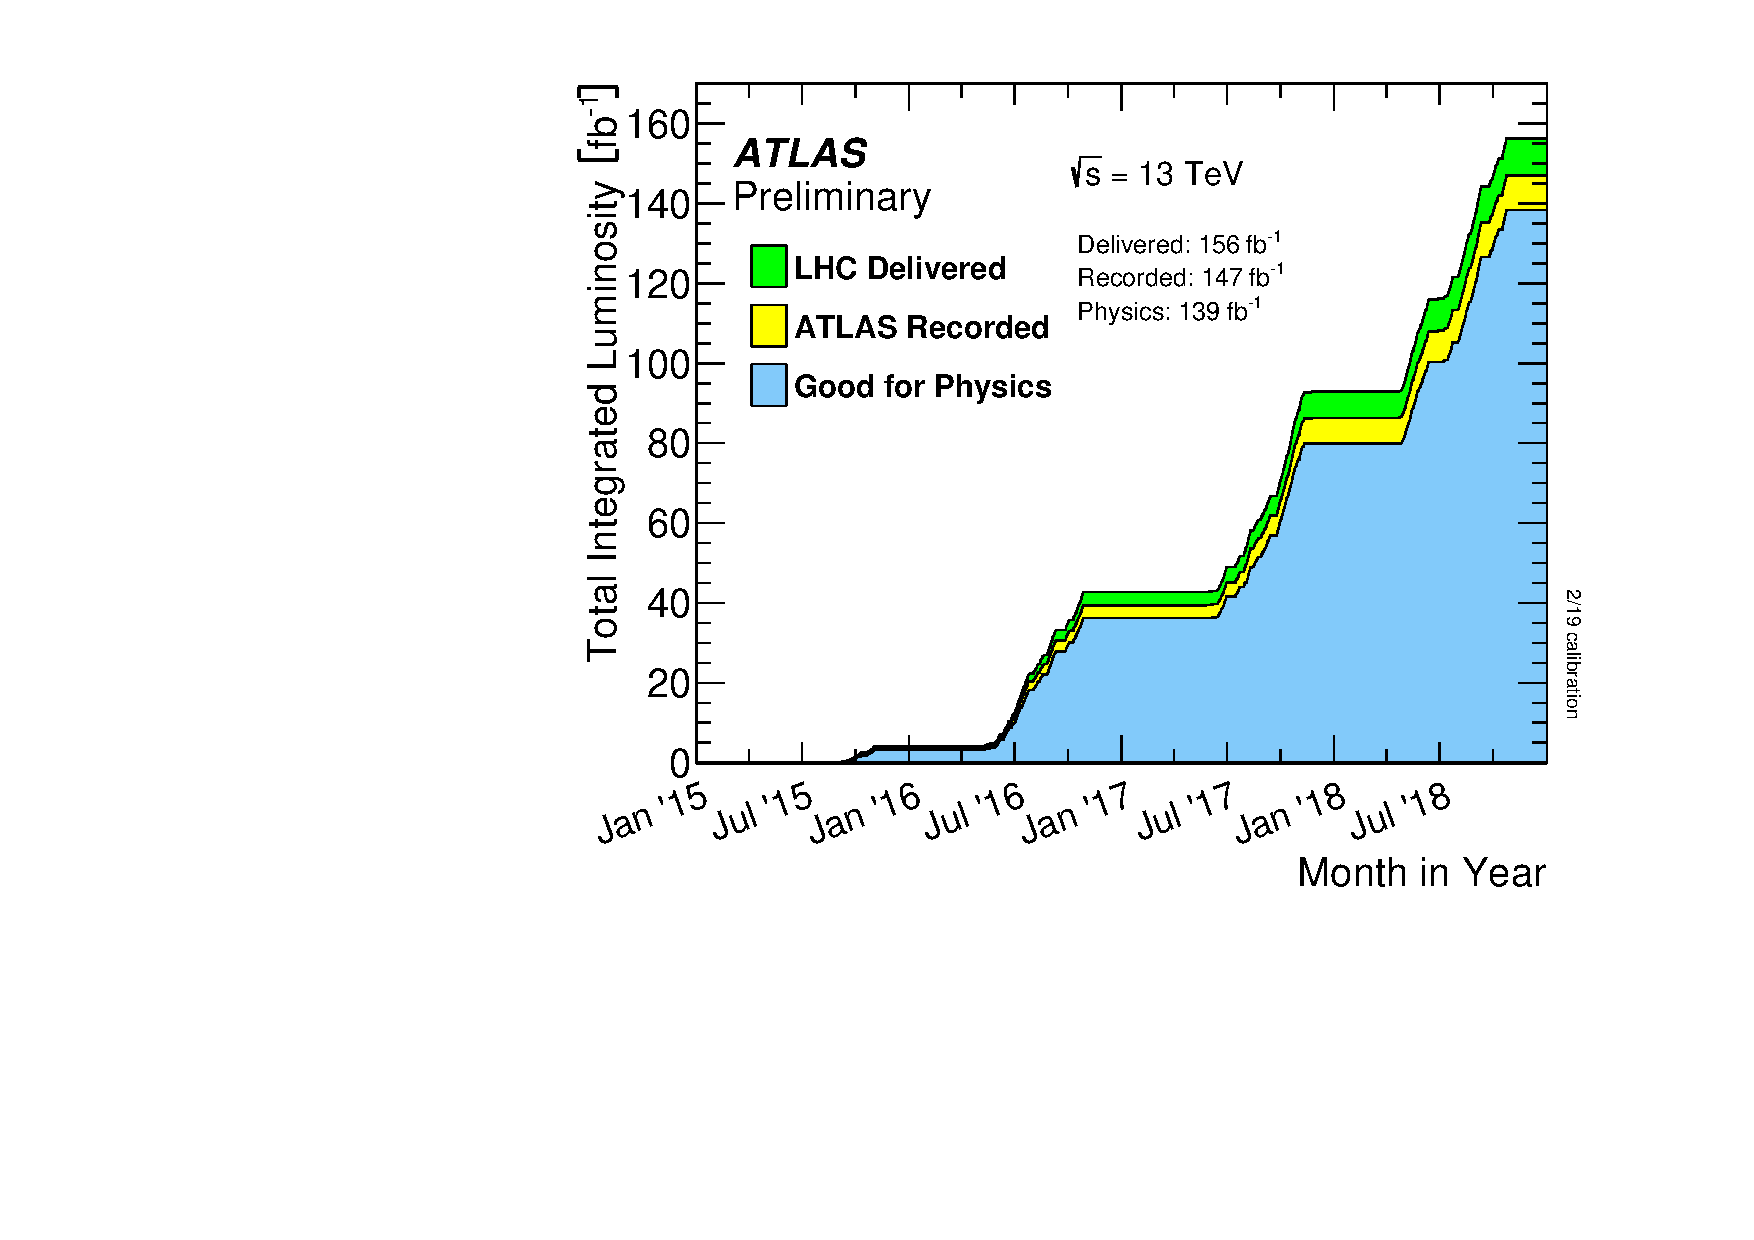
\includegraphics[width=\textwidth]{intlumivstimeRun2DQall}
		\caption{\label{fig:intlumivstimeRun2DQall}}
	\end{subfigure}%
	\caption{Instantaneous and cumulative luminosities in Run~2. Figure~\subref{fig:peakLumiByFill} shows the peak instantaneous luminosity delivered to ATLAS during $pp$ collision data taking in 2018 as a function of time. Figure~\subref{fig:intlumivstimeRun2DQall} shows the cumulative luminosity delivered to ATLAS (green), recorded by ATLAS (yellow) and deemed good for physics analysis (blue) during the entirety of Run~2~\cite{ATLAS:Run2}.}\label{fig:lumi_run2}
\end{figure}

Apart from the beam energy, the most important quantity for a collider is the instantaneous luminosity $L$. For a synchrotron with Gaussian beam distribution, the instantaneous luminosity can be written as
\begin{equation}
	L = \frac{N_b^2 n_b f_\mathrm{rev}}{4\pi\sigma_x\sigma_y} F,
	\label{eq:lumi}
\end{equation}
where $n_b$ is the number of bunches, $N_b$ the number of protons per bunch, $f_\mathrm{rev}$ the revolution frequency and $\sigma_x$ and $\sigma_y$ the transverse beam sizes. The parameters $F$ is a geometrical correction factor accounting for the reduction in instantaneous luminosity due to the beams crossing at a certain crossing angle. While the design instantaneous luminosity of the LHC at the high-luminosity experiments ATLAS and CMS is $L = \SI{e34}{\per\cm\squared\per\second}$~\cite{Evans:1129806}, the 2017 and 2018 data-taking periods saw a peak luminosity twice as high~\cite{peak_lumi}.

The instantaneous luminosity is related to the total number of events $N$ through the cross section $\sigma$ of the events in question
\begin{equation}
	N = \sigma L_\mathrm{int} = \sigma \int L\diff t,
\end{equation}
with $L_\mathrm{int}$ the total integrated luminosity, a measure for the total amount of collision data produced.

A precise knowledge of the integrated luminosity corresponding to a given dataset is crucial for both SM measurements as well as searches for BSM physics. Searches for SUSY like the one presented in this work rely on precise measurements of the integrated luminosity in order to be able to estimate the contribution from SM background processes. The luminosity measurement for the Run~2 dataset used within this work is described in detail in~\cite{ATLAS-CONF-2019-021,Aaboud:2016hhf} and relies on a measurement of the bunch luminosity, \ie the luminosity produced by a single pair of colliding bunches
\begin{equation}
	L_b = \frac{\mu f_\mathrm{rev}}{	\sigma_\mathrm{inel}} = \frac{\mu_\mathrm{vis}f_\mathrm{rev}}{\sigma_\mathrm{vis}},
\end{equation}
with $\mu$ the pile-up parameter, $\sigma_\mathrm{inel}$ the cross section of inelastic $pp$ collisions, $\mu_\mathrm{vis} = \epsilon \mu$ is the fraction $\epsilon$ of the pile-up parameter $\mu$ visible to the detector and $\sigma_\mathrm{vis} = \epsilon\sigma_\mathrm{inel}$ the visible inelastic cross section. If $\sigma_\mathrm{vis}$ is known, the currently recorded luminosity can be determined by measuring $\mu_\mathrm{vis}$. At the ATLAS experiment, the observed number of inelastic interactions per bunch crossing $\mu\mathrm{vis}$ is measured using dedicated detectors, as for example LUCID-2~\cite{Avoni_2018}, a forward Cherenkov-detector using the quartz windows from photomultipliers as Cherenkov medium.
In order to use $\mu_\mathrm{vis}$ as luminosity monitor, the respective detectors need to be calibrated through a measurement of the visible inelastic cross section $\sigma_\mathrm{vis}$. This can be done using van der Meer (vdM) scans~\cite{vanderMeer:296752,GRAFSTROM201597}, in which the transverse distribution of protons in the bunches is inferred by measuring the relative interaction rates as a function of the transverse beam separation\footnote{Often called \textit{beam sweeping}.}. The algorithms used to determine the $\sigma_\mathrm{vis}$ calibration are described in~\cite{ATLAS-CONF-2019-021,Aaboud:2016hhf} and the luminosity during the vdM runs can be determined using~\cref{eq:lumi}. At the LHC, vdM scans are typically performed in special low-$\mu$ runs with well-known machine parameters in order to minimise uncertainties~\cite{ATLAS-CONF-2019-021}. During high-$\mu$ physics runs, the luminosity measurement is then an extrapolation from the vdM runs.

The LHC entered operation in 2008, with first beams in September and first collisions by the end of November that same year~\cite{startup}. Its operation is in general structured into so-called \textit{Runs}, that are spanned by multiple years of data-taking. Run~1 spanned from 2009 to 2013 and delivered roughly $\SI{28.5}{\per\femto\barn}$ of $pp$ collision data to ATLAS, taken at centre-of-mass energies of $\SI{7}{\TeV}$ and $\SI{8}{\TeV}$~\cite{Aad:2011dr,Aad:1517411,Aaboud:2016hhf}. Run~2 lasted from 2015 to 2018 and saw a centre-of-mass energy increase to $\SI{13}{\TeV}$, delivering approximately $\SI{156}{\per\femto\barn}$ of $pp$ collision data to ATLAS~\cite{ATLAS-CONF-2019-021}. Run~3 of $pp$ collision data taking with two times design peak luminosity is currently planned to start its physics program in 2022 and last until end of 2024~\cite{run3}. Current plans foresee Run~3 to deliver about $\SI{150}{\per\femto\barn}$ of $pp$ collision data with centre-of-mass energies of $\SI{13}{\TeV}$ and $\SI{14}{\TeV}$. After Run~3, the LHC will be upgraded to the High Luminosity LHC, significantly increasing the peak instantaneous luminosity and delivering up to $\SI{3000}{\per\femto\barn}$ of $pp$ collision data from 2027 until 2040~\cite{run3,Apollinari:2284929}. 

This work uses $pp$ collision data taken by ATLAS during Run~2 of the LHC. Of the $\SI{156}{\per\femto\barn}$ delivered to ATLAS, $\SI{147}{\per\femto\barn}$ were recorded, and $\SI{139}{\per\femto\barn}$ were deemed to be good for physics analysis. \Cref{fig:lumi_run2} shows the cumulative luminosity delivered to ATLAS during Run~2. Uncertainties on the measurement total recorded luminosity stem from the measurements of $\mu_\mathrm{vis}$ and $\sigma_\mathrm{vis}$, but are dominated by the uncertainties on $\sigma_\mathrm{vis}$ as vdM scans can only be done during special runs, while the general conditions during high-$\mu$ conditions change continuously. For the full Run~2 dataset, the uncertainties accumulate to $\pm 1.7 \%$~\cite{ATLAS-CONF-2019-021}.

\section{ATLAS Experiment}\label{sec:atlas_experiment}

The ATLAS experiment is one of two general-purpose detectors at the LHC. Located at Point~1 in a cavern $\SI{100}{\meter}$ below the surface, it is approximately $\SI{44}{\meter}$ long and $\SI{25}{\meter}$ high~\cite{Aad:2008zzm}. The design of the ATLAS experiment is driven by the aim to allow for a diverse research program, including SM precision measurements, Higgs physics and searches for BSM physics, whilst at the same time taking into account the unique and challenging conditions set by the LHC. The various detector technologies used are designed to withstand the high-radiation environment of the LHC, while allowing particle measurements with high spatial and temporal granularity. The general structure of ATLAS is depicted in \cref{fig:atlas_detector}, and consists of a central part, called \textit{barrel}, that has a cylindrical shape around the beam pipe, and two discs, called \textit{end-caps}, that close off the barrel on each side. This makes the ATLAS detector forward-backward symmetric and covering nearly the full solid angle of $4\pi$, which is needed in order to measure momentum imbalances caused by particles that only interact weakly with the detector material.

The following sections introduce the working principles of the different detector components used in ATLAS, starting with the innermost component closest to the interaction point, the inner detector, followed by the calorimeters in the middle and finally the muon spectrometers on the outside. If not otherwise stated, details on the detector components are extracted from~\cite{Aad:2008zzm}.

\begin{figure}
	\centering    
	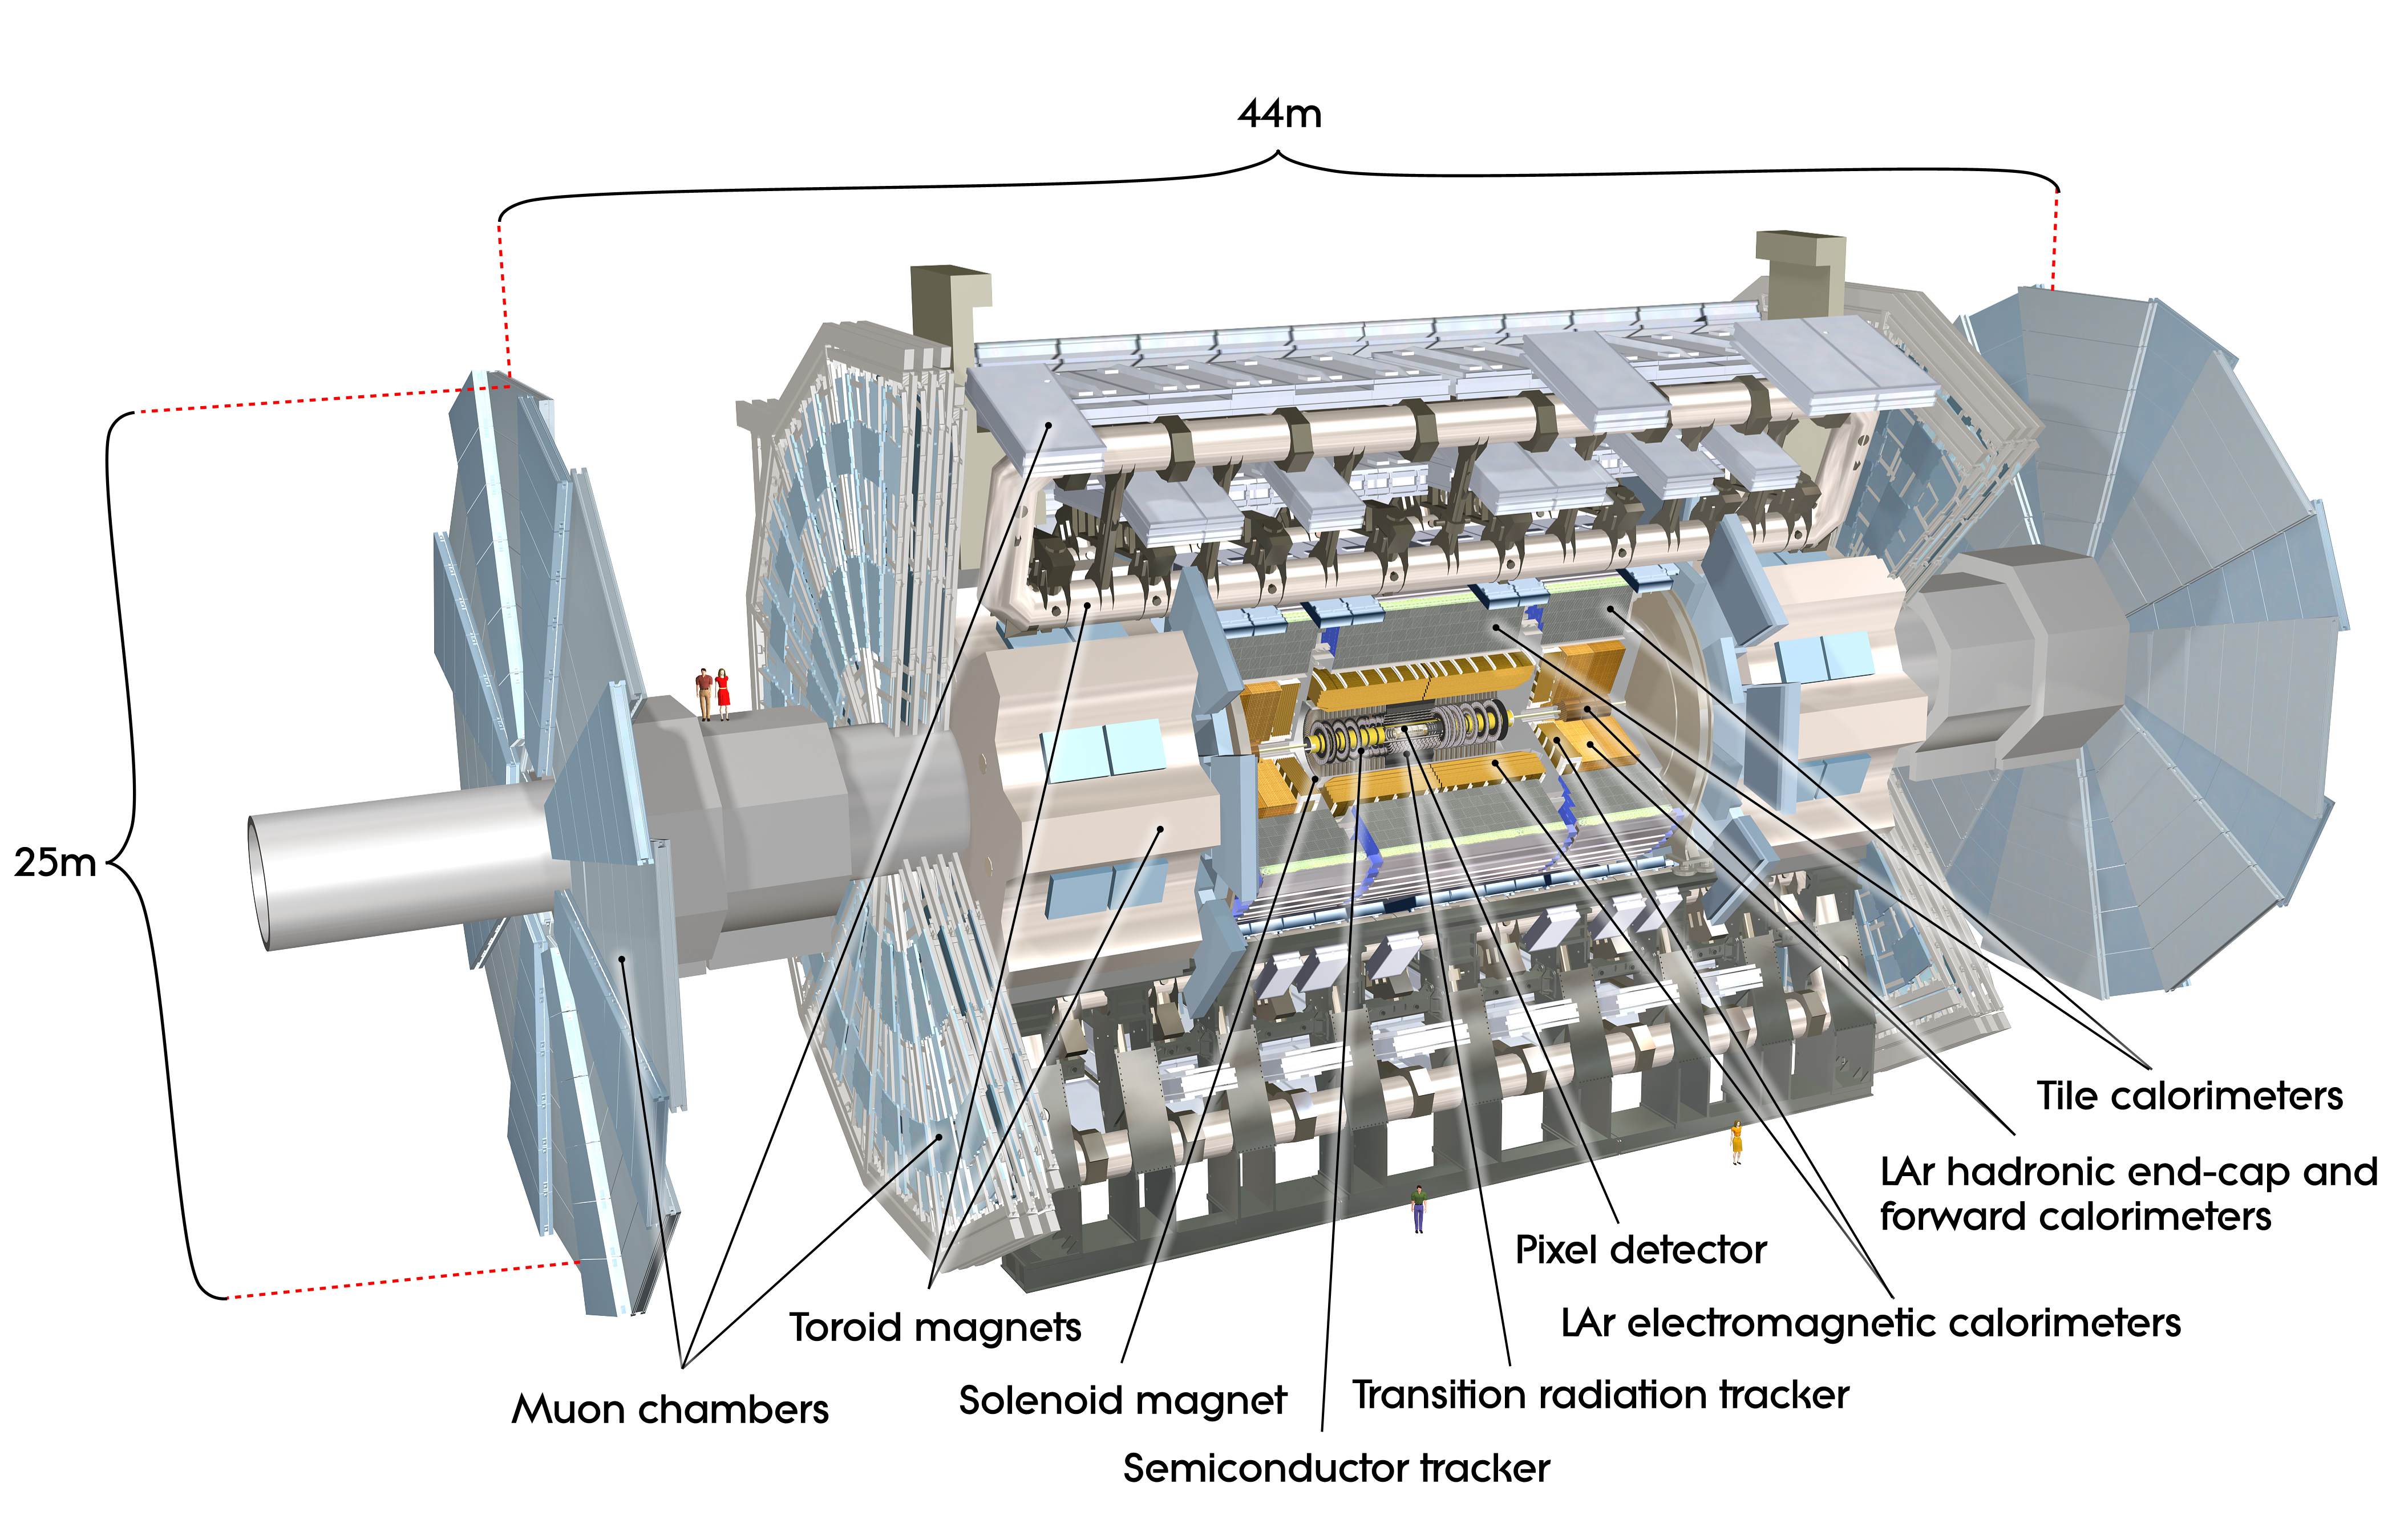
\includegraphics[width=0.9\textwidth]{atlas}
	\caption[The ATLAS detector]{Computer generated picture of the ATLAS detector, giving an overview on the various subsystems~\cite{Pequenao:1095924}.}
	\label{fig:atlas_detector}
\end{figure}


\subsection{Coordinate system}

In order to properly describe collision events in the ATLAS detector, a suitable detector system is needed. The right-handed coordinate system~\cite{ATLAS:1999uwa} used in ATLAS has its origin at the nominal interaction point in the centre of the detector. The positive $x$-axis points towards the centre of the LHC ring, the positive $y$-axis points upwards to the surface, and the beam pipe is used to define the $z$-axis. In the $x$--$y$ plane, called the transverse plane, the azimuthal angle $\phi$ is the angle around the beam axis, and the polar angle $\theta$ is measured from the beam axis. The rapidity~\cite{pdg2020} is defined as
\begin{equation}
	y = \frac{1}{2}\ln\left(\frac{E+p_z}{E-p_z}\right) = \tanh{\frac{p_z}{E}}^{-1},
\end{equation}
with $E$ the energy of an object and $p_z$ its momentum in $z$-direction. As opposed to the polar angle $\theta$, differences in the rapidity are invariant under Lorentz boosts in $z$-direction.

The pseudorapidity \cite{pdg2020} is the high-energy limit ($p\gg m$) of the rapidity, and defined as
\begin{align}
	\eta = - \ln\tan\frac{\theta}{2},
\end{align}
with $\cos\theta = p_z/p$. Pseudorapidity and rapidity are approximately equal in the limit where $p\gg m$ and $\theta \gg \frac{1}{\gamma}$. Compared to the rapidity, the pseudorapidity has the advantage of not depending on the energy and momentum calibration of the detected objects. Additionally, it gives a direct correspondence to the polar angle $\theta$ through the relation $\tanh\eta = \cos\theta$.

The distance between two objects in the ATLAS detector is given by
\begin{align}
	\Delta R=\sqrt{\left(\Delta \eta\right)^2+\left(\Delta \phi\right)^2}.
\end{align}
The longitudinal momentum of the partons composing the colliding hadrons is only known by means of the parton distribution functions (PDFs), stating the probabilities of the partons to have a certain energy in the direction of the beam. Thus, the total longitudinal energy in each collision is not exactly known, impeding the use of physics quantities in the $z$-direction. In the $x$--$y$ plane, however, momentum conservation can be applied, which is why mainly transverse physics quantities are used, indicated by a subscript `T', \eg $E_T$ or $p_T$.


\subsection{Magnet system}

\subsection{Inner detector}

\subsection{Calorimeters}

\subsection{Muon spectrometer}

\subsection{Forward detectors}

\subsection{Trigger and data acquisition system}

\subsection{Object reconstruction}


\section{Monte Carlo simulation}

